\section{Class Diagrams}
Class Diagrams describe the static structure of the system. Following classes diagram represent the relationship between different classes in OpenSCAD:
\begin{enumerate}
	\item Figure \ref{fig:classabstractnodecollgraph} shows the class diagram of the AbstractNode which is the basic class for all the nodes in the tree.
	\item Figure \ref{fig:collaborative} shows the Inheritanc Diagram of AbstractNode which shows all the classes inherited by AbstractNode.
	\item Figure \ref{fig:classprogresswidgetinheritgraph}  shows the Inheritance diagram of the ProgressWidget which show the amount of work done.
\end{enumerate}

\begin{figure}
\centering
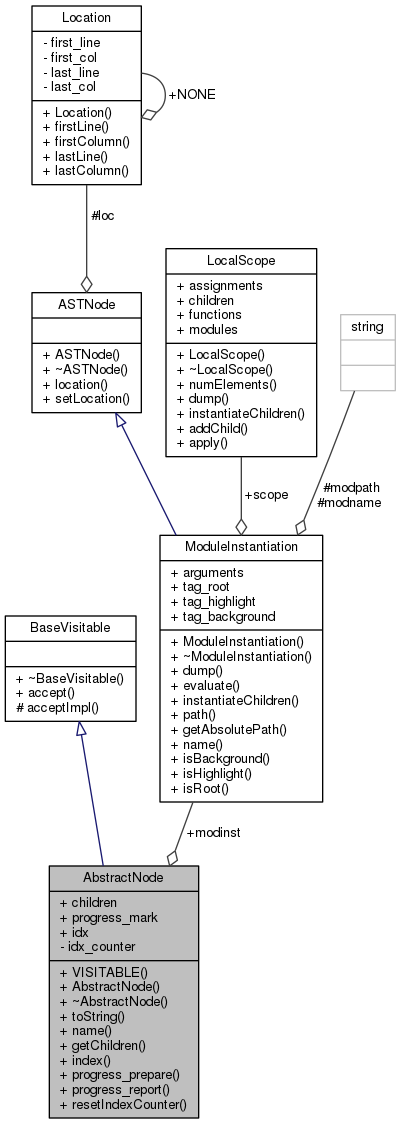
\includegraphics[width=0.5\linewidth]{images/classAbstractNode__coll__graph}
\caption{Class diagram of AbstractNode}
\label{fig:classabstractnodecollgraph}
\end{figure}

\begin{figure}
\centering
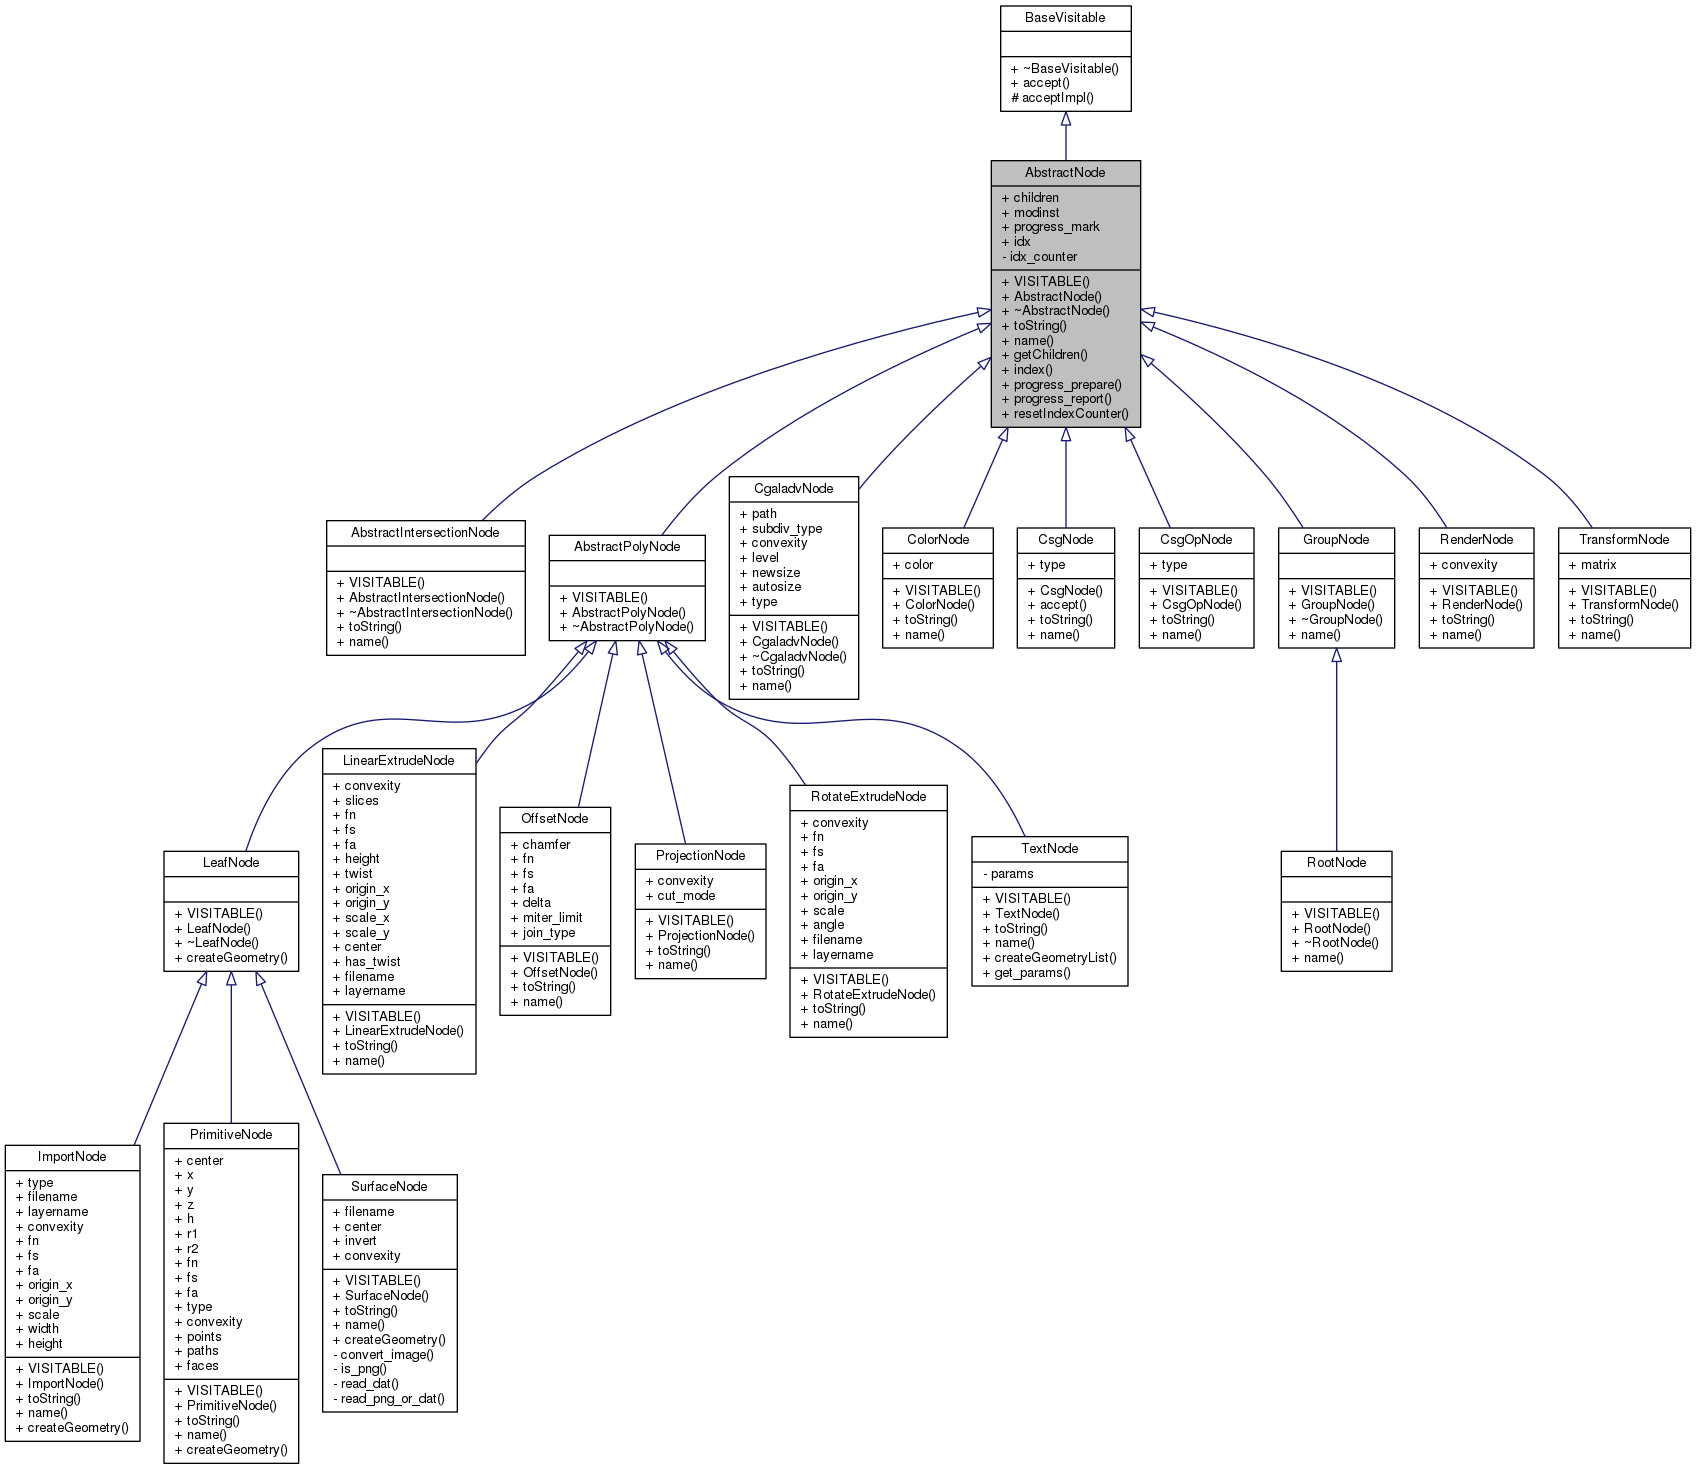
\includegraphics[width=\linewidth,height=1.37\columnwidth]{images/classAbstractNode__inherit__graph}
\caption{Inheritance graph of AbstractNode}
\label{fig:classabstractnodeinheritgraph}
\end{figure}


\begin{figure}
\centering
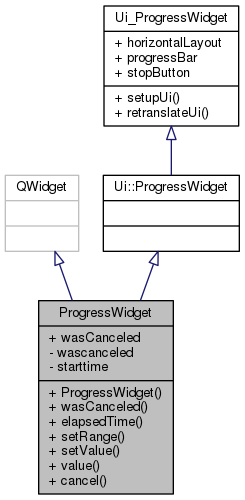
\includegraphics[width=0.4\linewidth]{images/classProgressWidget__inherit__graph}
\caption{Inheritance graph of ProgressWidget}
\label{fig:classprogresswidgetinheritgraph}
\end{figure}

